\documentclass{article}
%%%%%%% PACKAGES %%%%%%%%
\usepackage[utf8]{inputenc}
\usepackage{graphicx}
\usepackage{geometry}
\geometry{a4paper, margin=1in}
\usepackage{hyperref}
\usepackage{titling}
\usepackage{caption}
\usepackage{subcaption}
\usepackage{float}
\hypersetup{
    colorlinks=true,
    linkcolor=blue,
    filecolor=magenta,      
    urlcolor=cyan,
}

\title{Assignment 2: Swarm Intelligence\\CS 451: Computational Intelligence}
\author{Ali Asghar Yousuf $\mid$ Muhammad Murtaza}
\date{\today}

\begin{document}

\maketitle

\section{Ant Colony Optimization}

\subsection*{\begin{center}
  Capacitated Vehicle Routing Problem
\end{center}}

Plot of the best and average solution of Capacitated Vehicle Routing Problem using Ant Colony Optimization. The best solution is the one with the least distance. The average solution is the average of the distance of all the solutions in the population in each iteration.
\begin{figure}[H]
  \centering
  \textbf{Dataset A-n32-k5}
  \begin{subfigure}{.5\textwidth}
    \centering
    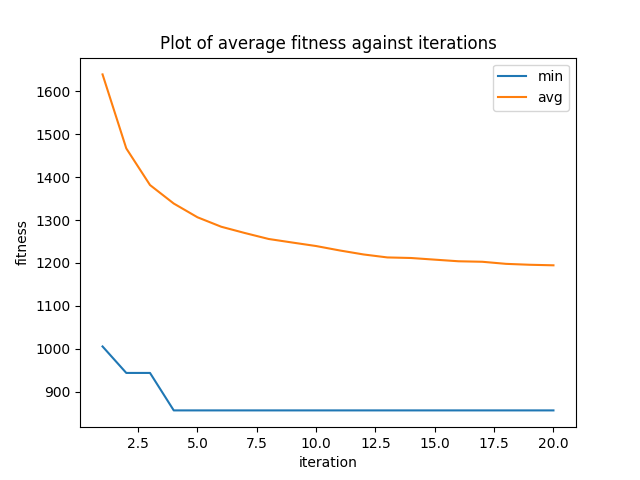
\includegraphics[width=1\linewidth]{images/n32-k5_20.png}
    \caption{ACO with 20 iterations}
    \label{fig:n32-k5_20}
  \end{subfigure}%
  \begin{subfigure}{.5\textwidth}
    \centering
    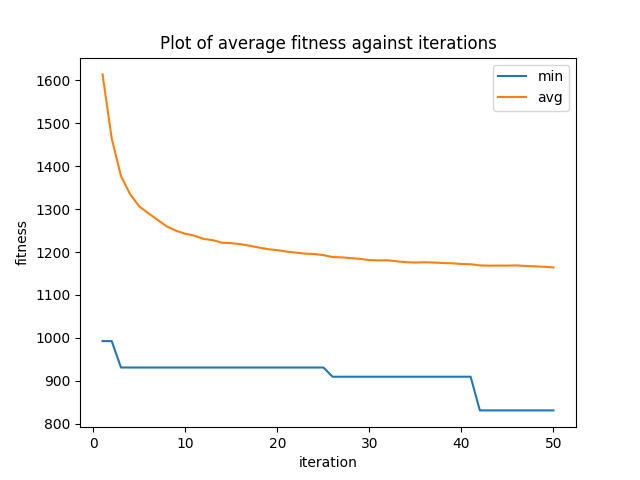
\includegraphics[width=1\linewidth]{images/n32-k5_50.png}
    \caption{ACO with 50 iterations}
    \label{fig:n32-k5_50}
  \end{subfigure}
  \caption{Note: Fitness is the distance}
  \label{fig:n32-k5}
\end{figure}

\begin{figure}[H]
  \centering
  \textbf{Dataset A-n44-k6}
  \begin{subfigure}{.5\textwidth}
    \centering
    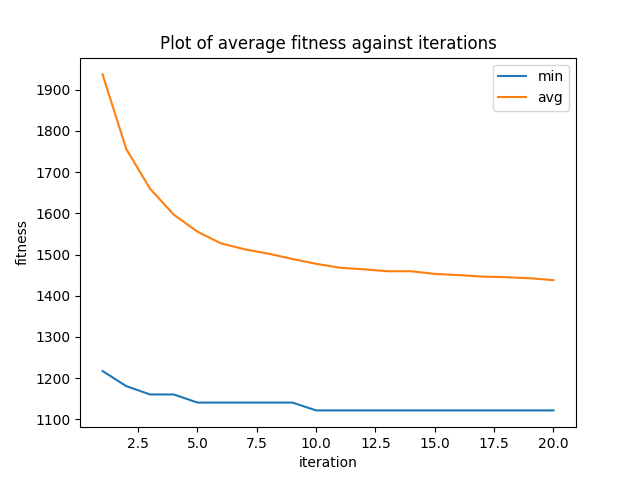
\includegraphics[width=1\linewidth]{images/n44-k6_20.png}
    \caption{ACO with 20 iterations}
    \label{fig:n44-k6_20}
  \end{subfigure}%
  \begin{subfigure}{.5\textwidth}
    \centering
    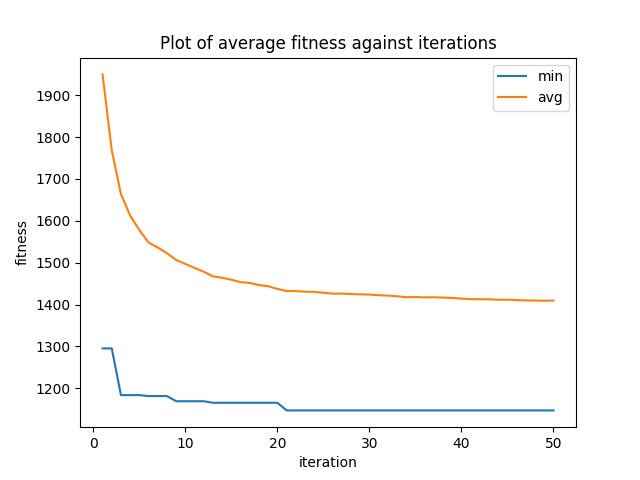
\includegraphics[width=1\linewidth]{images/n44-k6_50.png}
    \caption{ACO with 50 iterations}
    \label{fig:n44-k6_50}
  \end{subfigure}
  \caption{Note: Fitness is the distance}
  \label{fig:n44-k6}
\end{figure}

\begin{figure}[H]
  \centering
  \textbf{Dataset A-n60-k9}
  \begin{subfigure}{.5\textwidth}
    \centering
    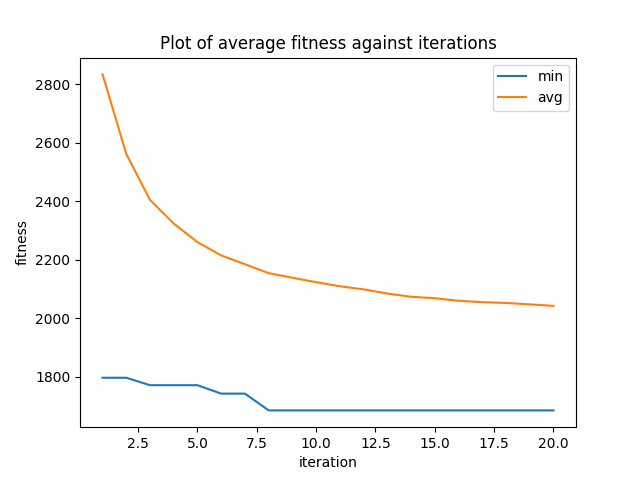
\includegraphics[width=1\linewidth]{images/n60-k9_20.png}
    \caption{ACO with 20 iterations}
    \label{fig:n60-k9_20}
  \end{subfigure}%
  \begin{subfigure}{.5\textwidth}
    \centering
    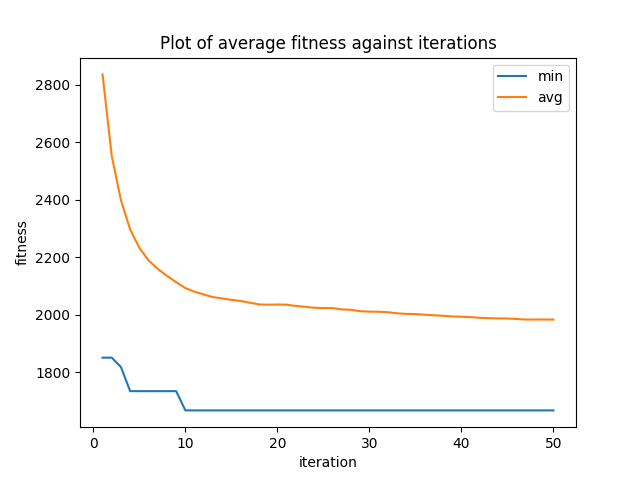
\includegraphics[width=1\linewidth]{images/n60-k9_50.png}
    \caption{ACO with 50 iterations}
    \label{fig:n60-k9_50}
  \end{subfigure}
  \caption{Note: Fitness is the distance}
  \label{fig:60-k9}
\end{figure}

\begin{figure}[H]
  \centering
  \textbf{Dataset A-n80-k10}
  \begin{subfigure}{.5\textwidth}
    \centering
    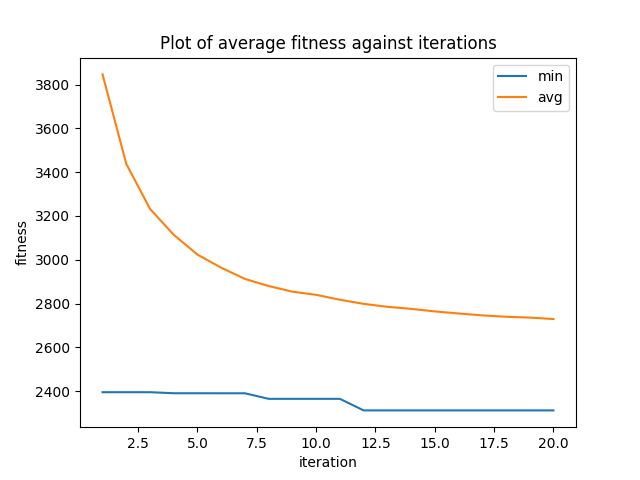
\includegraphics[width=1\linewidth]{images/n80-k10_20.png}
    \caption{ACO with 20 iterations}
    \label{fig:n80-k10_20}
  \end{subfigure}%
  \begin{subfigure}{.5\textwidth}
    \centering
    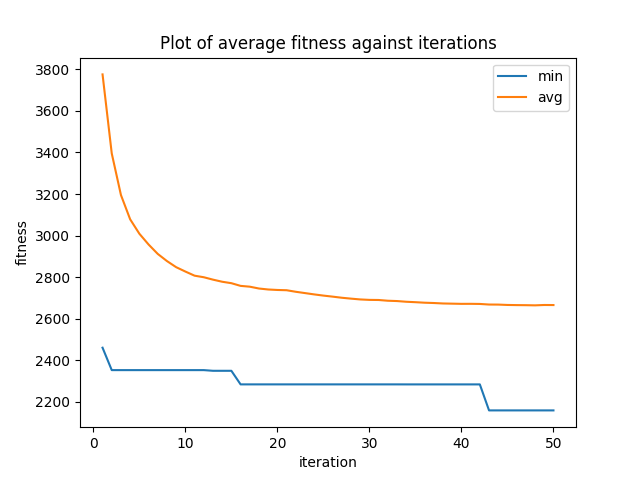
\includegraphics[width=1\linewidth]{images/n80-k10_50.png}
    \caption{ACO with 50 iterations}
    \label{fig:n80-k10_50}
  \end{subfigure}
  \caption{Note: Fitness is the distance}
  \label{fig:n80-k10}
\end{figure}

\section{Visualizing Swarms}

\subsection*{\begin{center}
  Visualizing Smoke Particle from Car Exhaust System
\end{center}}

\textbf{Given the current climate change events, it is important to create awareness of our daily carbon footprint, so we have made this smoke simulator that will aware people of how a car can damage our atmosphere, while at the same time we can represent particle system with it.}
\\~\\
Particle System is a collection of many minute particles that together represent a fuzzy object. Here we have a smoke particles that together will represent smoke from car exhaust system. 

\begin{figure}[H]
  \centering
    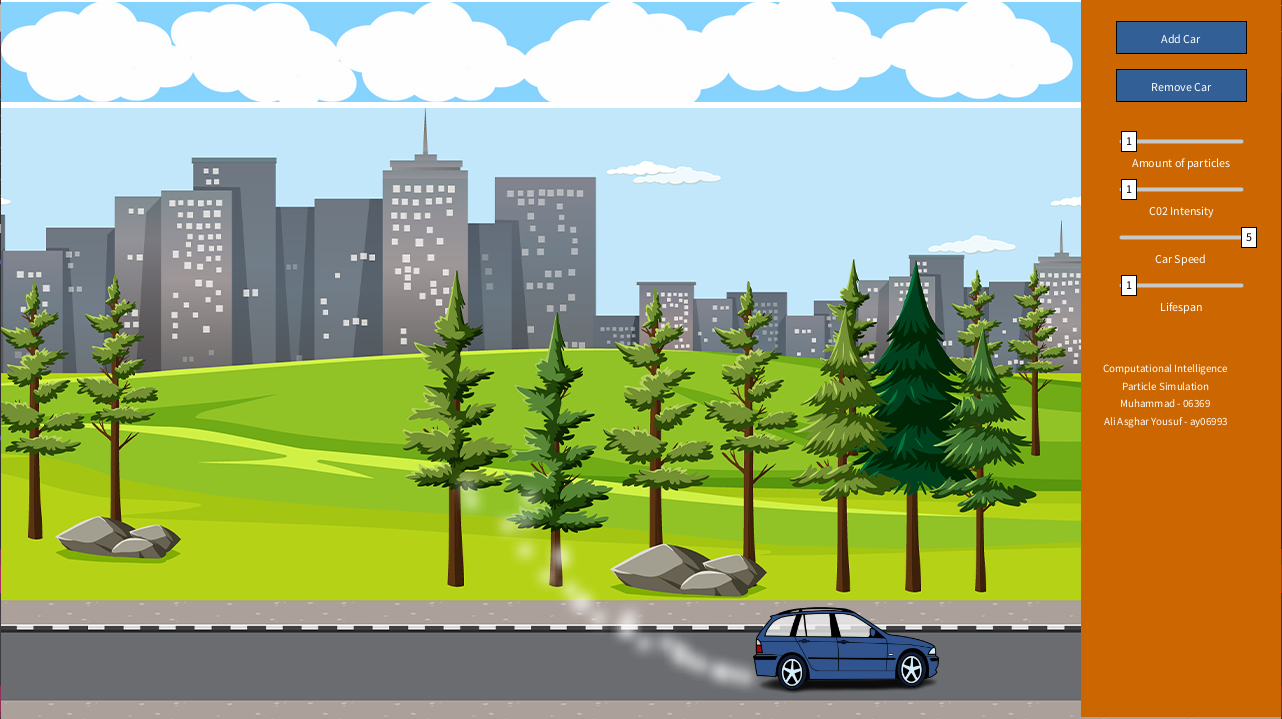
\includegraphics[width=1\linewidth]{images/simulator.png}
    \caption{Car Exhaust Smoke Simulator}
\end{figure}

\textbf{First we will classify all the attributes of a particle system}
\\
\begin{itemize}
  \item Position: Each particle has a given position on the screen with 'x' and 'y' coordinate.
  \item Velocity: Each particle has a randomly generated velocity which is constant. 
  \item Lifetime: Life of a particle can be changed in this system. When a life of particle ends, it dies from the system. 
  \item Color: Initially it is white, if the CO2 intensity increases, it becomes black.
  \item Shape: The particle has round shape.
  \item Size: 16 pixels.
\end{itemize}

\textbf{Each of the following phases of particles has been implemented in this system}
\begin{itemize}
    \item Particle Lifespan
    \begin{itemize}
      \item{Each particle is generated randomly in each iteration}
      \item{Particles moves upwards towards the sky.}
      \item{Particle is rendered on the screen on each given position}
      \item{Particle then reaches extinction phase when it dies from the system}
    \end{itemize}
    \item Particle Generation
    \begin{itemize}
      \item{Particle is generated in each iteration of the system randomly. We can control particle generation by increasing or decreasing its chances of generation in the given system.}
    \end{itemize}
    \item Particle Dynamics
    \begin{itemize}
      \item{The particle has a position vector and it is moved by adding the corresponding velocity vector to it.}
      \item{The particle has a zero acceleration and its velocity is kept constant. However acceleration can be added to velocity.}
    \end{itemize}
    \item Extinction
\end{itemize}

\textbf{The video of the simulation can be seen here: }
\href{https://www.youtube.com/watch?v=BU9WsN1110Y}{https://www.youtube.com/watch?v=BU9WsN1110Y}


\end{document}
